\documentclass[11pt]{article}

% ============================================================
%  QAARIB — Backend Architecture & Orchestration Flowchart
%  Compiles with: pdflatex qaarib_architecture.tex  (run twice)
% ============================================================

\usepackage[a4paper,margin=1.2cm]{geometry}
\usepackage{tikz}
\usepackage{amsmath}
\usepackage{helvet}
\renewcommand{\familydefault}{\sfdefault}

\usetikzlibrary{shapes.geometric, arrows.meta, positioning, calc, backgrounds, fit, decorations.pathreplacing}

% ----- Palette (Qatar maroon + Fanar charcoal + metro line accents) -----
\definecolor{maroon}{HTML}{8A1538}      % Qatar maroon
\definecolor{ink}{HTML}{1A1A1A}
\definecolor{paper}{HTML}{FAF7F2}
\definecolor{slate}{HTML}{2A2A2A}
\definecolor{detgreen}{HTML}{00A14B}    % metro Green = deterministic / no model
\definecolor{detgreenbg}{HTML}{E8F6EE}
\definecolor{toolblue}{HTML}{1F6FEB}
\definecolor{toolbluebg}{HTML}{E7F0FD}
\definecolor{fanargold}{HTML}{B8860B}   % gold = model reached (costly)
\definecolor{fanargoldbg}{HTML}{F8F0DA}
\definecolor{redline}{HTML}{D6001C}
\definecolor{mute}{HTML}{6B6B6B}
\definecolor{cardbg}{HTML}{FFFFFF}

% ----- Node styles -----
\tikzset{
  io/.style       = {rectangle, rounded corners=3pt, draw=ink, line width=0.8pt,
                      fill=white, text width=3.5cm, align=center, font=\footnotesize\bfseries,
                      minimum height=0.9cm, inner sep=4pt},
  det/.style      = {rectangle, rounded corners=4pt, draw=detgreen, line width=1.1pt,
                      fill=detgreenbg, text width=8.6cm, align=left, font=\footnotesize,
                      inner sep=7pt},
  tool/.style     = {rectangle, rounded corners=4pt, draw=toolblue, line width=1.1pt,
                      fill=toolbluebg, text width=8.6cm, align=left, font=\footnotesize,
                      inner sep=7pt},
  model/.style    = {rectangle, rounded corners=4pt, draw=fanargold, line width=1.1pt,
                      fill=fanargoldbg, text width=8.6cm, align=left, font=\footnotesize,
                      inner sep=7pt},
  decision/.style = {diamond, aspect=2.2, draw=maroon, line width=1pt, fill=white,
                      align=center, font=\scriptsize\bfseries, inner sep=1pt, text width=2.2cm},
  exit/.style     = {rectangle, rounded corners=10pt, draw=detgreen, line width=1pt,
                      fill=white, font=\scriptsize\bfseries, text=detgreen,
                      inner sep=4pt, align=center},
  flow/.style     = {-{Stealth[length=2.4mm]}, line width=0.9pt, draw=slate},
  flowyes/.style  = {-{Stealth[length=2.4mm]}, line width=0.9pt, draw=detgreen},
  flowno/.style   = {-{Stealth[length=2.4mm]}, line width=0.9pt, draw=maroon},
  stagelabel/.style = {font=\scriptsize\bfseries\sffamily, text=mute},
}

\pagestyle{empty}

\begin{document}

% =====================================================================
%  HEADER
% =====================================================================
\begin{center}
  {\color{maroon}\rule{\textwidth}{2pt}}\\[4pt]
  {\Huge\bfseries\color{maroon} Qaarib}\\[2pt]
  {\large\bfseries\color{ink} Backend Orchestration Architecture}\\[3pt]
  {\footnotesize\color{mute} A Qatar-local agentic assistant on the Fanar platform \;$\cdot$\; Fanar Hackathon 2026}\\[2pt]
  {\color{maroon}\rule{\textwidth}{2pt}}
\end{center}

\vspace{0pt}

% =====================================================================
%  USP BANNER  (the embedded unique selling point)
% =====================================================================
\begin{center}
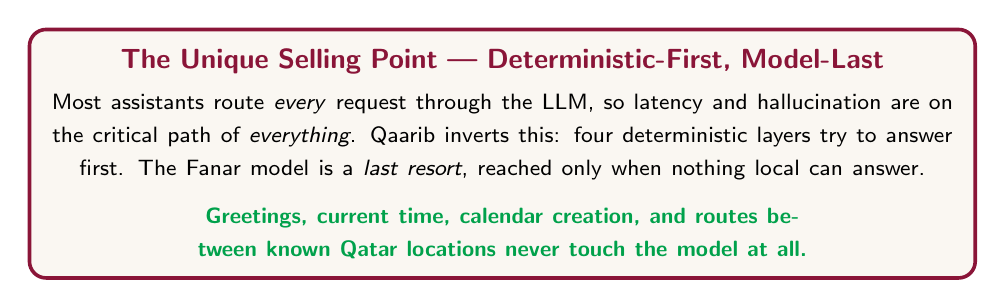
\begin{tikzpicture}
  \node[rectangle, rounded corners=6pt, draw=maroon, line width=1.3pt,
        fill=paper, text width=0.95\textwidth, align=center, inner sep=7pt] {
    {\bfseries\color{maroon} The Unique Selling Point — Deterministic-First, Model-Last}\\[3pt]
    {\footnotesize Most assistants route \emph{every} request through the LLM, so latency and
    hallucination are on the critical path of \emph{everything}. Qaarib inverts this: four
    deterministic layers try to answer first. The Fanar model is a \emph{last resort},
    reached only when nothing local can answer.}\\[5pt]
    {\footnotesize\bfseries\color{detgreen} Greetings, current time, calendar creation, and routes
    between known Qatar locations never touch the model at all.}
  };
\end{tikzpicture}
\end{center}

\vspace{2pt}

% =====================================================================
%  MAIN FLOWCHART
% =====================================================================
\begin{center}
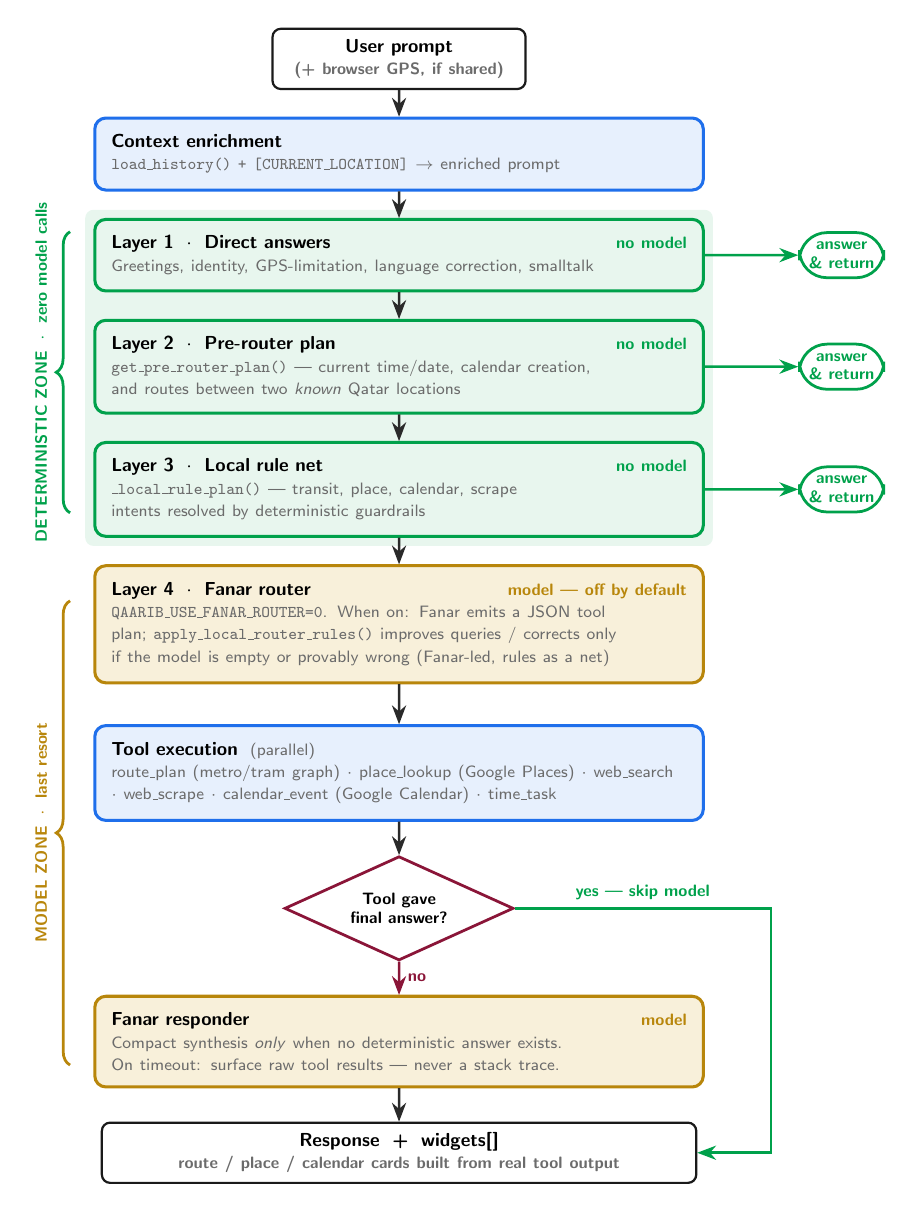
\begin{tikzpicture}[node distance=4mm and 9mm, scale=0.85, transform shape]

% ---- Entry ----
\node[io] (user) {User prompt\\ \textcolor{mute}{\scriptsize (+ browser GPS, if shared)}};

% ---- L0: Context enrichment ----
\node[tool, below=of user, text width=8.6cm] (ctx)
  {\textbf{Context enrichment}\\
   \textcolor{mute}{\scriptsize\texttt{load\_history() + [CURRENT\_LOCATION]} $\rightarrow$ enriched prompt}};

% ---- L1: Direct answers ----
\node[det, below=of ctx] (l1)
  {\textbf{Layer 1 \;$\cdot$\; Direct answers} \hfill {\scriptsize\color{detgreen}\bfseries no model}\\
   \textcolor{mute}{\scriptsize Greetings, identity, GPS-limitation, language correction, smalltalk}};

% ---- L2: Pre-router deterministic plan ----
\node[det, below=of l1] (l2)
  {\textbf{Layer 2 \;$\cdot$\; Pre-router plan} \hfill {\scriptsize\color{detgreen}\bfseries no model}\\
   \textcolor{mute}{\scriptsize\texttt{get\_pre\_router\_plan()} — current time/date, calendar creation,}\\
   \textcolor{mute}{\scriptsize and routes between two \emph{known} Qatar locations}};

% ---- L3: Local rule plan ----
\node[det, below=of l2] (l3)
  {\textbf{Layer 3 \;$\cdot$\; Local rule net} \hfill {\scriptsize\color{detgreen}\bfseries no model}\\
   \textcolor{mute}{\scriptsize\texttt{\_local\_rule\_plan()} — transit, place, calendar, scrape}\\
   \textcolor{mute}{\scriptsize intents resolved by deterministic guardrails}};

% ---- L4: Fanar router (optional / off by default) ----
\node[model, below=of l3] (l4)
  {\textbf{Layer 4 \;$\cdot$\; Fanar router} \hfill {\scriptsize\color{fanargold}\bfseries model — off by default}\\
   \textcolor{mute}{\scriptsize\texttt{QAARIB\_USE\_FANAR\_ROUTER=0}. When on: Fanar emits a JSON tool}\\
   \textcolor{mute}{\scriptsize plan; \texttt{apply\_local\_router\_rules()} improves queries / corrects only}\\
   \textcolor{mute}{\scriptsize if the model is empty or provably wrong (Fanar-led, rules as a net)}};

% ---- Tools ----
\node[tool, below=6mm of l4] (tools)
  {\textbf{Tool execution} \;\textcolor{mute}{\scriptsize(parallel)}\\
   \textcolor{mute}{\scriptsize route\_plan (metro/tram graph) $\cdot$ place\_lookup (Google Places) $\cdot$ web\_search}\\
   \textcolor{mute}{\scriptsize $\cdot$ web\_scrape $\cdot$ calendar\_event (Google Calendar) $\cdot$ time\_task}};

% ---- Deterministic bypass ----
\node[decision, below=5mm of tools] (det2) {Tool gave\\ final answer?};

% ---- Responder ----
\node[model, below=5mm of det2] (resp)
  {\textbf{Fanar responder} \hfill {\scriptsize\color{fanargold}\bfseries model}\\
   \textcolor{mute}{\scriptsize Compact synthesis \emph{only} when no deterministic answer exists.}\\
   \textcolor{mute}{\scriptsize On timeout: surface raw tool results — never a stack trace.}};

% ---- Output ----
\node[io, below=5mm of resp, text width=8.6cm] (out)
  {Response \;+\; \textbf{widgets[]}\\
   \textcolor{mute}{\scriptsize route / place / calendar cards built from \emph{real} tool output}};

% ===== Vertical spine arrows =====
\draw[flow] (user) -- (ctx);
\draw[flow] (ctx)  -- (l1);
\draw[flow] (l1)   -- (l2);
\draw[flow] (l2)   -- (l3);
\draw[flow] (l3)   -- (l4);
\draw[flow] (l4)   -- (tools);
\draw[flow] (tools)-- (det2);
\draw[flowno]  (det2) -- node[right, font=\scriptsize\bfseries, text=maroon] {no} (resp);
\draw[flow] (resp) -- (out);

% ===== Early-exit arrows (each deterministic layer can short-circuit) =====
\node[exit, right=14mm of l1] (e1) {answer\\ \& return};
\node[exit, right=14mm of l2] (e2) {answer\\ \& return};
\node[exit, right=14mm of l3] (e3) {answer\\ \& return};
\draw[flowyes] (l1.east) -- (e1) ;
\draw[flowyes] (l2.east) -- (e2) ;
\draw[flowyes] (l3.east) -- (e3) ;

% deterministic bypass YES arrow (skip responder)
\draw[flowyes] (det2.east) -| ($(out.east)+(1.1,0)$)
      node[pos=0.25, above, font=\scriptsize\bfseries, text=detgreen] {yes — skip model}
      -- (out.east);

% ===== The "cost spine" brace : how far down before the model is touched =====
\begin{scope}[on background layer]
  \node[rectangle, fill=detgreenbg, rounded corners=3pt,
        fit=(l1)(l2)(l3), inner sep=3pt] (detzone) {};
\end{scope}
\draw[decorate, decoration={brace, amplitude=5pt, mirror}, line width=1pt, draw=detgreen]
     ($(l1.west)+(-0.35,0.35)$) -- ($(l3.west)+(-0.35,-0.35)$)
     node[midway, left=6pt, align=center, font=\scriptsize\bfseries, text=detgreen, rotate=90, anchor=south]
     {DETERMINISTIC ZONE \;$\cdot$\; zero model calls};

\draw[decorate, decoration={brace, amplitude=5pt, mirror}, line width=1pt, draw=fanargold]
     ($(l4.west)+(-0.35,0.35)$) -- ($(resp.west)+(-0.35,-0.35)$)
     node[midway, left=6pt, align=center, font=\scriptsize\bfseries, text=fanargold, rotate=90, anchor=south]
     {MODEL ZONE \;$\cdot$\; last resort};

\end{tikzpicture}
\end{center}

\vspace{-2pt}

% =====================================================================
%  FOOTER LEGEND
% =====================================================================
\begin{center}
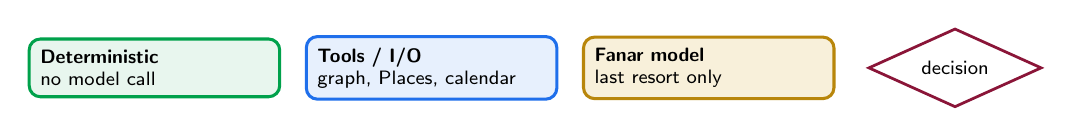
\begin{tikzpicture}[node distance=3mm]
  \node[det, text width=2.9cm, font=\scriptsize, inner sep=4pt] (lg1) {\textbf{Deterministic}\\ no model call};
  \node[tool, right=3mm of lg1, text width=2.9cm, font=\scriptsize, inner sep=4pt] (lg2) {\textbf{Tools / I/O}\\ graph, Places, calendar};
  \node[model, right=3mm of lg2, text width=2.9cm, font=\scriptsize, inner sep=4pt] (lg3) {\textbf{Fanar model}\\ last resort only};
  \node[decision, right=4mm of lg3, text width=1.6cm, font=\scriptsize] (lg4) {decision};
\end{tikzpicture}
\end{center}

\vspace{-4pt}
\begin{center}
{\scriptsize\color{mute}
Reliability by design: each deterministic layer returns immediately on a hit, so
model latency and hallucination are removed from the critical path of the most common
Qatar-local tasks. If Fanar is slow or unreachable, the deterministic zone still answers.}
\end{center}

\end{document}
